\clearpage
\section{Standard Model backgrounds}
There are three main types of SM background to new physics search in the di-electron channel. The most significant is the irreducible SM Drell-Yan process. New physics can interfere with this process, if not mitigated, the effects can be significant.

The second most important background type comes from electrons from non-singularly produced W and Z bosons. The dominant source of these electrons are from \ttbar\ events although $WW$ events become increasingly important at high mass as the boost of the top quark means that the b-jet enters the electrons isolation cone and so the electron fails isolation requirements. Other sources include $tW$, $WZ$, $ZZ$ and \ztt\ events although they are small compared to \ttbar\ and $WW$, mainly entering at the Z peak. This background is referred to \ttbar\ and \ttbar-like background as it is dominated by \ttbar.

The third background is the jet background, where one or more jets is misidentified as an electron, mainly arising from $W$+jets and multijets where one more jets is reconstructed as an electron.

\subsection{SM Drell-Yan background}

The SM Drell-Yan background is estimated using simulated events generated by the POWHEG event generator interfaced to PYTHIA8.
Like all previous analyses, the Monte Carlo samples are normalised to the data in Z peak region of 60-120~\GeVCSq unless otherwise stated. They are also corrected with the trigger turn on curve.
Figure~\ref{fig:Zpeak} shows the data and MC at the Z peak for the barrel-barrel and barrel-endcap. In this case, in order to see the normalisation agreement between data and MC, MC events are weighted to the luminosity, trigger turn on curve is applied and the scale factor between data and MC for gsf electron reconstruction efficiency and HEEP ID efficiency is applied. Further to this, official electron energy scale and smearing is applied for data and MC in order to get better data and MC agreement.


\begin{figure}[bh]
\begin{center}
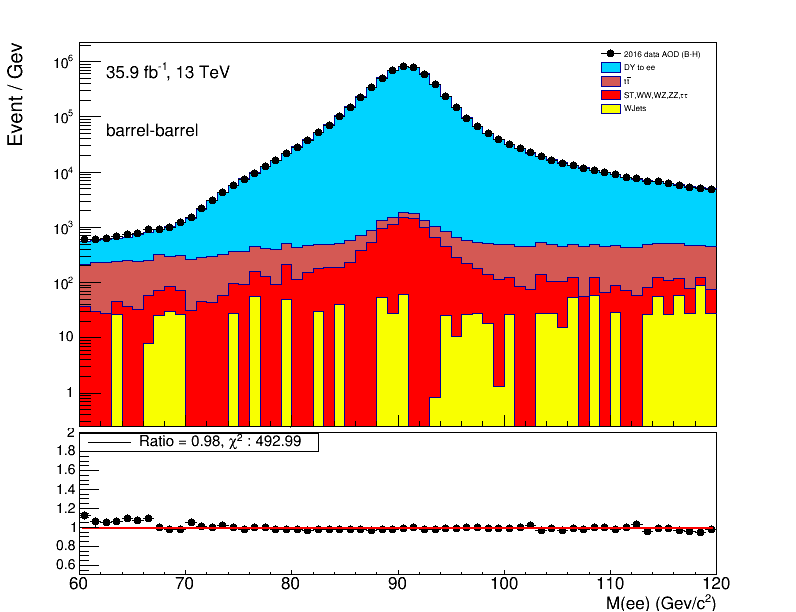
\includegraphics[angle=0,width=0.49\textwidth]{figures/Zprime/2016/zPeakDY/hratio_M_ee2__barrel-barrel.png}
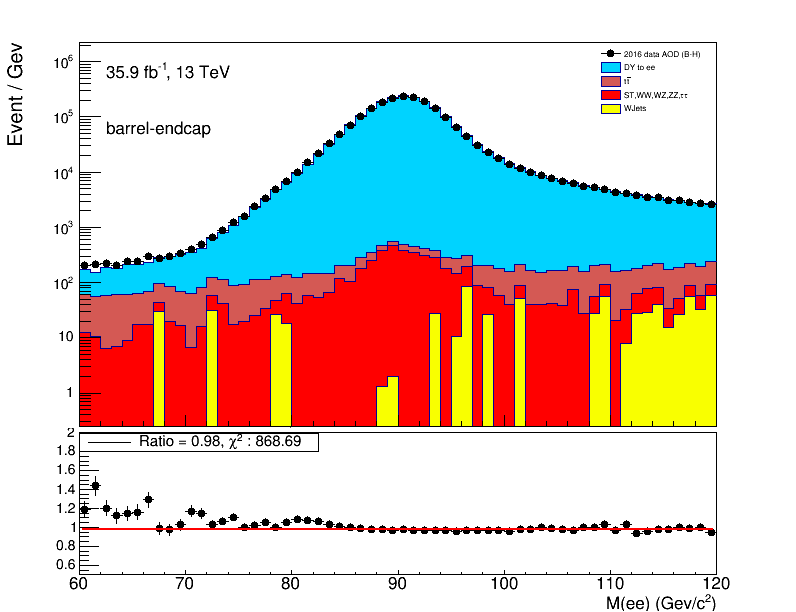
\includegraphics[angle=0,width=0.49\textwidth]{figures/Zprime/2016/zPeakDY/hratio_M_ee2__barrel-endcap.png}
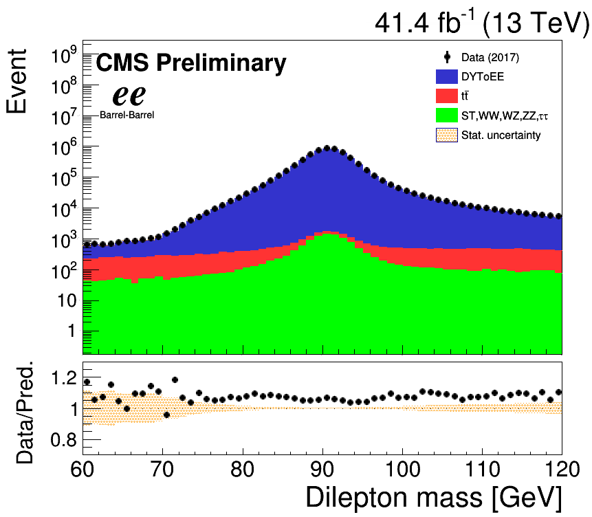
\includegraphics[angle=0,width=0.49\textwidth]{figures/Zprime/2017/zPeakDY/BB_hratio_M_ee.png}
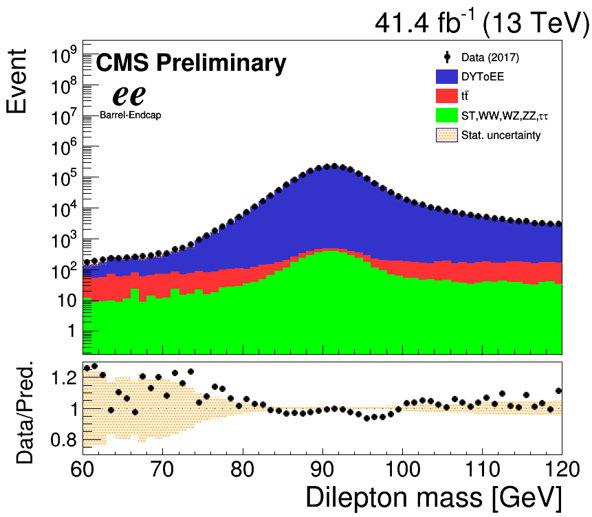
\includegraphics[angle=0,width=0.49\textwidth]{figures/Zprime/2017/zPeakDY/BE_hratio_M_ee.png}
\end{center}
\caption{Data - MC agreement in the Z peak region with the MC normalised to the luminosity of data for the barrel-barrel (left) and barrel-endcap (right) regions. The trigger turn on curve, gsf reconstruction and HEEP ID scale factor are applied for MC in 2016 (top) and 2017 (bottom).}
\label{fig:Zpeak}
\end{figure}

A cross-section measurement including the trigger efficiencies and data/MC efficiency scale factors is shown in table~\ref{bkg:tab:zCrossSec}.
The SM Z cross section in mass range 60 to 120 GeV at NNLO is 1928$\pm72$ pb.
The result has a good agreement with theory value. it is $\sim$2\% for barrel-barrel and $\sim$0.3\% for barrel-endcap in 2016, for 2017 it is $\sim$2\% for barrel-barrel and $\sim$4\% for barrel-endcap.
\begin{table}[!hbt]
\begin{center}
\resizebox{\linewidth}{!}{%
\begin{tabular}{|c|c|c|c|c|} \hline
Year                    & \multicolumn{2}{c|}{2016}                 & \multicolumn{2}{c|}{2017|} \\ \hline
Channel                 & barrel-barrel                     & barrel-endcap           & barrel-barrel                & barrel-endcap   \\\hline
N data events           & 5760345$\pm$2400                  & 2051759$\pm$1432        & 6189746$\pm$2488             & 2095959$\pm$1448\\
N expect bkg            & 32805                             & 11336                   & 32092                        & 10540           \\
MC acc$\times$eff       & 0.0880$\pm$0.001(stat.)           & 0.0315$\pm$0.001(stat.) & 0.0807$\pm$0.001(stat.)      & 0.0289$\pm$0.001(stat.)\\
Data/MC gsf RECO SF     & 0.979$\pm$X                       & 0.985$\pm$X             &  -                           &  -                     \\
Data/MC ID Eff SF       & 0.943$\pm$0.001(stat.)            & 0.953$\pm$0.002(stat.)  & 0.935$\pm$0.002(stat.)       & 0.947$\pm$0.004(stat.) \\\hline
Luminosity (\invpb)     & 35867                             & 35867                   & 41368                        & 41368                  \\
DY cross-section (pb)   & 1967$\pm$3(stat)$\pm$51(lumi)     & 1922$\pm$3(stat)$\pm$50(lumi) & 1974$\pm$3(stat)       & 1854$\pm$3(stat)   \\\hline
Ratio to theory (1928 pb)&1.02                              &0.997                          &1.024                   &0.962                \\\hline
\end{tabular}}
\caption{The DY cross-section measurement in the range of $60<M_{ee}<120$~\GeVCSq. The HEEP efficiency data/MC scale factor is taken from table~\ref{tab:HEEP_eff_nominal}.
Note that in table~\ref{tab:HEEP_eff_nominal} the scale factors are for individual electrons while here they are for electron pairs. For 2017 the data/MC gsf electron reconstruction efficiency scale factor is already included in MC acc$\times$eff.}
\label{bkg:tab:zCrossSec}
\end{center}
\end{table}

\subsubsection{DY Background Correction and Uncertainty}
\label{sec:dyBkgCorr}
The main uncertainties on the Drell-Yan background originate from PDF and higher-order effects.
The cross-section has been evaluated using FEWZ 3.1.b2 with NNLO accuracy in QCD and NLO in EWK.
Photon induced effects were taken into account by using a special PDF set, namely the LUXqed\_plus\_PDF4LHC15\_nnlo\_100.
Cross section ratios relative to the Z peak were estimated together with their uncertainties by taking into account possible correlations
of the PDF uncertainties between the various mass bins. Full details of this calculation are in~\cite{AN-16-053}.
The cross-sections in various mass bins were evaluated in the analysis acceptance ($E_T>35$~GeV, $|\eta|<2.5$, excluding the $1.4442-1.566$ region).
The ratio of these cross-sections to that predicted by our POWHEG samples generated with NNPDF3.0 is shown in figure~\ref{fig:fewzPowheg}.

%It is immediately noted that the POWHEG NNPDF3.0 prediction is increasingly higher than the FEWZ prediction at as the mass increases.
%This appears to be related to the choice of PDFs, figure~\ref{fig:fewzMCATNLOCTVsNNPDF3Powheg} shows the ratio pf the POWHEG cross-section
%predictions when using CT10 and C14 other the prediction using NNPDF3.0. It should be noted that ATLAS in their 2015 result used CT10.
%Finally the prediction of mc@NLO is compared to POWHEG is also shown in figure~\ref{fig:fewzMCATNLOCTVsNNPDF3Powheg}.

It is immediately noted that the POWHEG NNPDF3.0 prediction is increasingly higher than the FEWZ prediction as the mass increases.
It is unclear what the analysis should do about this and current approach is to apply a FEWZ to POWHEG k-factor.
This would slightly improve data/MC agreement at high mass. The functional form for
this k-factor (accounting for the fact we normalise in the 60-120 GeV region) is shown
in figure~\ref{fig:fewzPowheg}. This is now applied in the mass spectrum plots and the background estimations for the limits.

The PDF uncertainties for FEWZ 3.1.b2 with the LUXqed\_plus\_PDF4LHC15\_nnlo\_100 PDF set are shown in table~\ref{bkg:tab:pdfUncert}.
The uncertainties quoted are on the ratio to the Z peak region of 60 to 120~GeV to the invariant mass region in question. The uncertainties are fitted by
polynomial which is shown in Figure \ref{fig:pdf_rel_uncert}.


\begin{figure}[bh]
\begin{center}
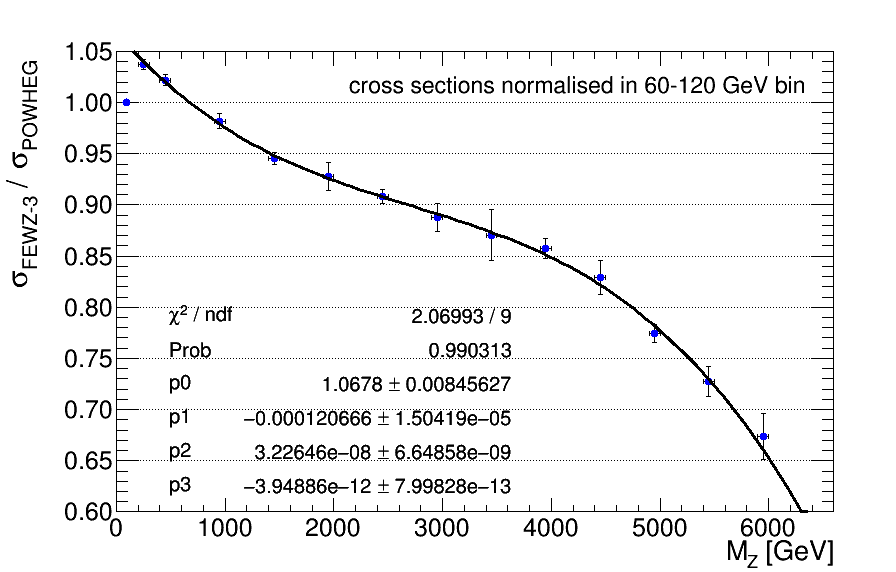
\includegraphics[angle=0,width=0.8\textwidth]{figures/Zprime/2016/zPeakDY/powhegFEWZKFactor.png}
\end{center}
\caption{
%The ratio of the \zee\ cross-section as predicted by FEWZ 3.1 at NNLO using the PDF4LHC15nnlo PDF set and that predicted by POWHEG at
%NLO using the NNPDF3.0 PDF set in various mass bins. The cross-sections are normalised to each other in the 60 to 120 GeV bin.
The ratio of the \zee\ cross-section as predicted by FEWZ 3.1.b2 using the LUXqed\_plus\_PDF4LHC15\_nnlo\_100 PDF set and that predicted by
POWHEG at NLO using the NNPDF3.0 PDF set in various mass bins. The cross-sections are normalised to each other in the 60 to 120 GeV bin.
}
\label{fig:fewzPowheg}
\end{figure}

%\begin{figure}[bh]
%\begin{center}
%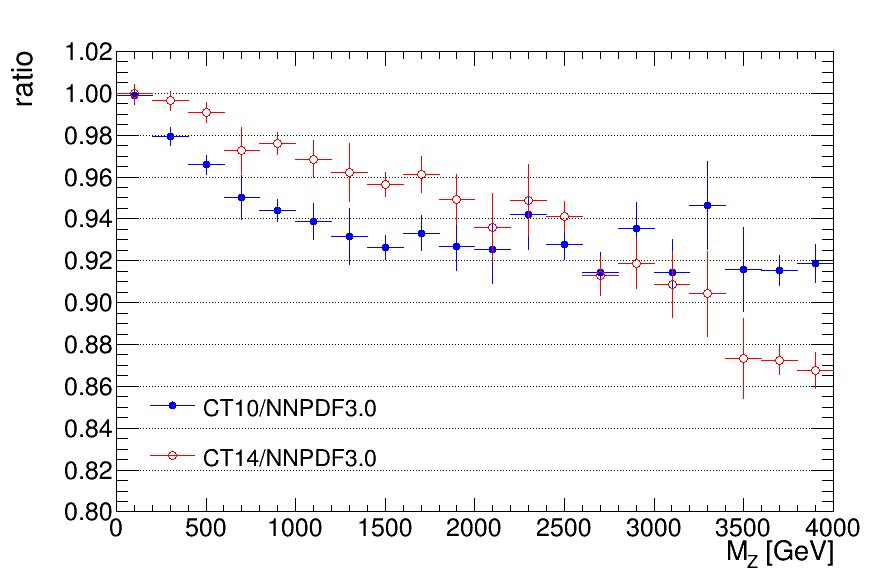
\includegraphics[angle=0,width=0.49\textwidth]{fig/fig_zPeakDY/ctOverNNPDF.png}
%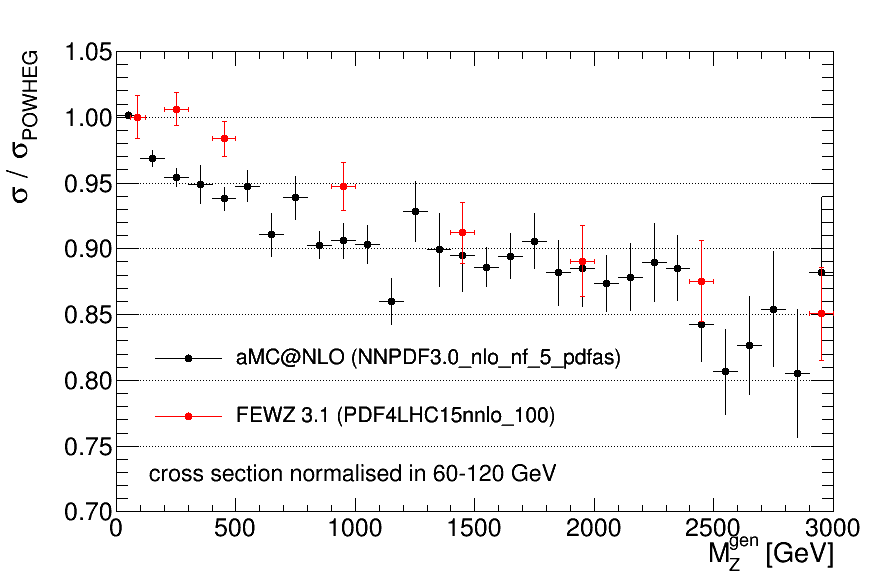
\includegraphics[angle=0,width=0.49\textwidth]{fig/fig_zPeakDY/mcatnloFewzVsPowheg}
%\end{center}
%\caption{
%The ratio of the \zee\ cross-section as predicted by FEWZ 3.1 at NNLO using the PDF4LHC15nnlo PDF set
%and as predicted by mc@NLO at NLO using the NNPDF3.0 PDF set to that predicted by POWHEG at NLO using the
%NNPDF3.0 PDF set in various mass bins. All cross-sections normalised to each other in the 60 to 120 GeV bin.
%}
%\label{fig:fewzMCATNLOCTVsNNPDF3Powheg}
%\end{figure}


\begin{table}[t]
\begin{center}
\smallskip\noindent
%\resizebox{\linewidth}{!}{%
\begin{tabular}{|c|c|} \hline
mass range (GeV) & relative uncertainty \\\hline
 200-300 & 1.21\% \\
 400-500 & 1.54\% \\
900-1000 & 2.16\% \\
1400-1500 & 2.73\% \\
1900-2000 & 3.24\% \\
2400-2500 & 3.72\% \\
2900-3000 & 4.27\% \\
3400-3500 & 5.00\% \\
3900-4000 & 5.94\% \\
4400-4500 & 7.47\% \\
4900-5000 & 10.2\% \\
5400-5500 & 14.3\% \\
5900-6000 & 19.9\% \\\hline
\end{tabular}%}
\caption{The PDF uncertainties relative to the Z peak region as a function of mass.
%These numbers are taken from Table 3 of AN-16-053 v3~\cite{AN-16-053}
}
\label{bkg:tab:pdfUncert}
\end{center}
\end{table}

\begin{figure}[bh]
\begin{center}
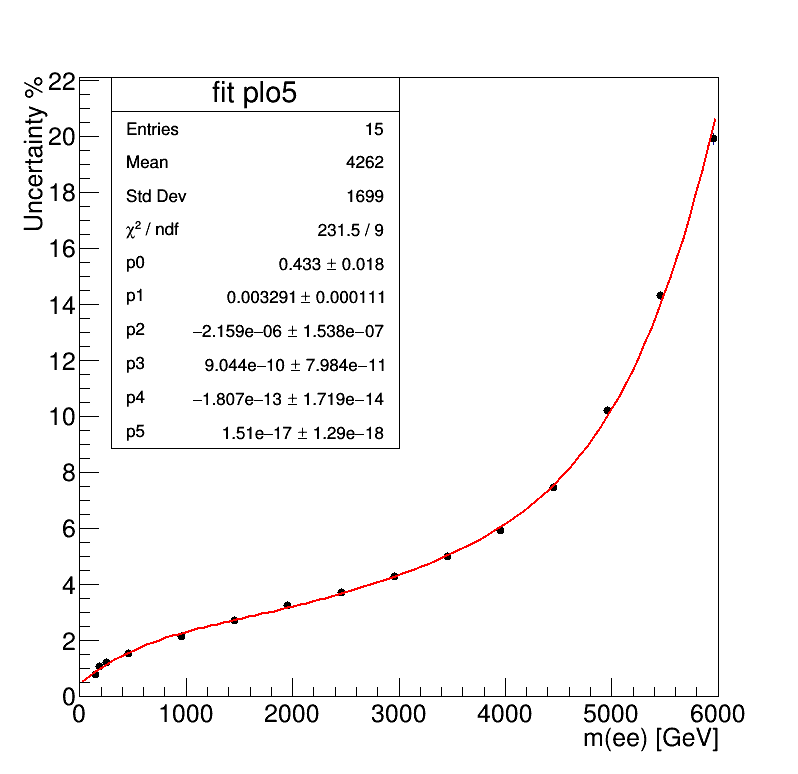
\includegraphics[angle=0,width=0.8\textwidth]{figures/Zprime/2016/pdf_uncert_relative.png}
\end{center}
\caption{
The PDF uncertainties relative to the Z peak region as a function of mass.
}
\label{fig:pdf_rel_uncert}
\end{figure}



\clearpage
